\documentclass[11pt,a4paper]{article}

\usepackage[margin=20mm,headheight=15pt]{geometry}

\usepackage{longtable,booktabs,array,hyperref,xcolor,tikz,fancyhdr}

\usepackage{fontspec,xeCJK}

\setmainfont[Ligatures=TeXOff]{Times New Roman}

\setsansfont[Ligatures=TeXOff]{Times New Roman}

\setmonofont[Ligatures=TeXOff,WordSpace={1,1,1}]{Times New Roman}

\setCJKmainfont{Noto Serif CJK SC}

\setCJKsansfont{Noto Serif CJK SC}

\setCJKmonofont{Noto Serif CJK SC}

\newfontfamily\vulcanmathsymbols{Noto Serif CJK SC}

\XeTeXgenerateactualtext=1

\definecolor{vulcan}{HTML}{BB3E23}

\pgfdeclarelayer{connections}\pgfdeclarelayer{edge labels}\pgfsetlayers{connections,main,edge labels}

\hypersetup{hidelinks}

\newcolumntype{L}[1]{>{\raggedright\arraybackslash}p{#1}}

\setlength{\emergencystretch}{5em}\tolerance=2000\hbadness=10000

\setlength{\parindent}{0pt}\setlength{\parskip}{5pt}

\pagestyle{fancy}\fancyhf{}\fancyhead[L]{\small\sffamily\textbf{VULCAN SILICON ENGINEERING}}

\fancyhead[R]{\small\sffamily Technical Design, Quartus STA \& FPGA Verification Report}\fancyfoot[C]{\small\sffamily Page \thepage}

\begin{document}

{\footnotesize\sffamily\textcolor{vulcan}{\textbf{VULCAN AUTONOMOUS CHIP DESIGN \& HARDWARE SIGNOFF SERIES \hfill DOCUMENT CLASS: ENGINEERING VERIFICATION REPORT}}\par}

\vspace{2pt}\textcolor{vulcan}{\rule{\textwidth}{1.2pt}}\vspace{4pt}

{\sffamily\LARGE\raggedright\textbf{RIVET-A3 Multi-Key,\allowbreak{} Multi-Context AES Cryptographic Subsystem}\par}

\vspace{4pt}

{\footnotesize\sffamily\renewcommand{\arraystretch}{1.22}\begin{tabular}{@{}L{0.22\textwidth}L{0.74\textwidth}@{}}\toprule\textbf{Author \& Contact} & Sufeng Guo (\allowbreak{}sufeng\_\allowbreak{}guo@smail.nju.edu.cn,\allowbreak{} v-sufengguo@microsoft.com)\allowbreak{}\\\textbf{Target Platform} & Intel Arria 10 GX (\texttt{10AX115N3F40E2SG}) \textemdash{} Microsoft Catapult Longs Peak (Bedrock 2.1)\\\textbf{Verification Stack} & Icarus Verilog 12.0 $\cdot$ Yosys 0.33 $\cdot$ Intel Quartus Prime 17.1 TimeQuest STA $\cdot$ PCIe Gen3x8 HIL\\\textbf{Release Timestamp} & 2026-10-19 23:41 UTC+\allowbreak{}8 (\allowbreak{}Beijing Time)\allowbreak{}\\\bottomrule\end{tabular}\par}

\vspace{4pt}

\begin{abstract}\noindent 

RIVET-A3 is a standalone SystemVerilog cryptographic subsystem supporting AES-128/\allowbreak{}256 ECB,\allowbreak{} CTR and GCM through legacy streaming,\allowbreak{} direct descriptors and descriptor DMA. Four hardware keyslots and four saved contexts enable interleaved GCM sessions without software handling intermediate cryptographic state. Authentication-gated payload retention prevents failed GCM decryption from releasing plaintext.


The behavioral campaign passed all nine combinations of capacities 1,\allowbreak{} 3 and 16 blocks with seeds 17,\allowbreak{} 89 and 203. Additional checks exercised the 256-block maximum,\allowbreak{} rejected illegal capacities,\allowbreak{} behaviorally detected a disposable cryptographic mutation and reproduced a focused campaign from copied deliverable sources. Default-capacity generic synthesis reported 2,\allowbreak{}200,\allowbreak{}117 generic primitive cells and zero inferred latches. These results establish bounded RTL functionality and generic synthesizability,\allowbreak{} not physical implementation or security certification.


\end{abstract}

\section{Architecture and design rationale}

A shared iterative AES engine and a 128-cycle polynomial GHASH multiplier serve a byte-serial session controller. Sharing avoids four replicated cryptographic engines while preserving arbitrary-byte GCM fragment boundaries. Four saved records preserve continuation state; separate payload banks retain output and destination ownership across descriptors. The scheduler owns DMA queues,\allowbreak{} descriptor fetching,\allowbreak{} memory transactions and completion delivery. Fully resettable storage favors explicit zeroization over technology-specific RAM inference. Blocks are arranged row-major in three columns; relationships represent concurrent control,\allowbreak{} data and ownership paths,\allowbreak{} not a serial pipeline. Architecture and implementation are documented by E001,\allowbreak{} E002 and E014.

\begin{center}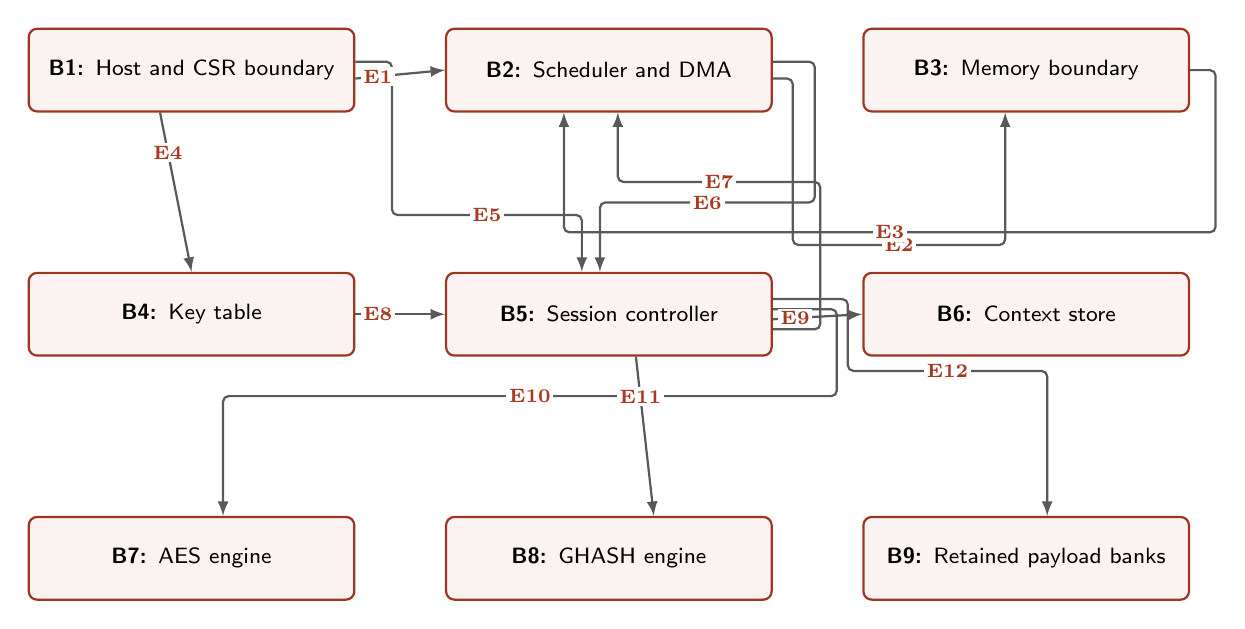
\begin{tikzpicture}[every node/.style={font=\footnotesize\sffamily},>=latex]

\node[draw=vulcan!85!black,thick,rounded corners=3pt,fill=vulcan!6,text width=3.9cm,minimum height=1.05cm,align=center] (b0) at (0.0,0.0) {\textbf{B1:} Host and CSR boundary};

\node[draw=vulcan!85!black,thick,rounded corners=3pt,fill=vulcan!6,text width=3.9cm,minimum height=1.05cm,align=center] (b1) at (5.3,0.0) {\textbf{B2:} Scheduler and DMA};

\node[draw=vulcan!85!black,thick,rounded corners=3pt,fill=vulcan!6,text width=3.9cm,minimum height=1.05cm,align=center] (b2) at (10.6,0.0) {\textbf{B3:} Memory boundary};

\node[draw=vulcan!85!black,thick,rounded corners=3pt,fill=vulcan!6,text width=3.9cm,minimum height=1.05cm,align=center] (b3) at (0.0,-3.1) {\textbf{B4:} Key table};

\node[draw=vulcan!85!black,thick,rounded corners=3pt,fill=vulcan!6,text width=3.9cm,minimum height=1.05cm,align=center] (b4) at (5.3,-3.1) {\textbf{B5:} Session controller};

\node[draw=vulcan!85!black,thick,rounded corners=3pt,fill=vulcan!6,text width=3.9cm,minimum height=1.05cm,align=center] (b5) at (10.6,-3.1) {\textbf{B6:} Context store};

\node[draw=vulcan!85!black,thick,rounded corners=3pt,fill=vulcan!6,text width=3.9cm,minimum height=1.05cm,align=center] (b6) at (0.0,-6.2) {\textbf{B7:} AES engine};

\node[draw=vulcan!85!black,thick,rounded corners=3pt,fill=vulcan!6,text width=3.9cm,minimum height=1.05cm,align=center] (b7) at (5.3,-6.2) {\textbf{B8:} GHASH engine};

\node[draw=vulcan!85!black,thick,rounded corners=3pt,fill=vulcan!6,text width=3.9cm,minimum height=1.05cm,align=center] (b8) at (10.6,-6.2) {\textbf{B9:} Retained payload banks};

\begin{pgfonlayer}{connections}

\draw[->,thick,black!65] ([yshift=-0.107cm]b0.east) -- coordinate[pos=0.25] (e0) ([yshift=0.000cm]b1.west);

\draw[->,thick,black!65,rounded corners=2pt] ([yshift=-0.107cm]b1.east) -- (7.635,-0.107) -- (7.635,-2.220) -- coordinate[midway] (e1) (10.333,-2.220) -- ([xshift=-0.267cm]b2.south);

\draw[->,thick,black!65,rounded corners=2pt] ([yshift=0.000cm]b2.east) -- (13.005,0.000) -- (13.005,-2.060) -- coordinate[midway] (e2) (4.729,-2.060) -- ([xshift=-0.571cm]b1.south);

\draw[->,thick,black!65] ([xshift=-0.400cm]b0.south) -- coordinate[pos=0.25] (e3) ([xshift=0.000cm]b3.north);

\draw[->,thick,black!65,rounded corners=2pt] ([yshift=0.107cm]b0.east) -- (2.545,0.107) -- (2.545,-1.840) -- coordinate[midway] (e4) (4.957,-1.840) -- ([xshift=-0.343cm]b4.north);

\draw[->,thick,black!65,rounded corners=2pt] ([yshift=0.107cm]b1.east) -- (7.915,0.107) -- (7.915,-1.680) -- coordinate[midway] (e5) (5.186,-1.680) -- ([xshift=-0.114cm]b4.north);

\draw[->,thick,black!65,rounded corners=2pt] ([yshift=-0.192cm]b4.east) -- (7.985,-3.292) -- (7.985,-1.420) -- coordinate[midway] (e6) (5.414,-1.420) -- ([xshift=0.114cm]b1.south);

\draw[->,thick,black!65] ([yshift=0.000cm]b3.east) -- coordinate[pos=0.25] (e7) ([yshift=0.000cm]b4.west);

\draw[->,thick,black!65] ([yshift=-0.064cm]b4.east) -- coordinate[pos=0.25] (e8) ([yshift=0.000cm]b5.west);

\draw[->,thick,black!65,rounded corners=2pt] ([yshift=0.064cm]b4.east) -- (8.195,-3.036) -- (8.195,-4.140) -- coordinate[midway] (e9) (0.400,-4.140) -- ([xshift=0.400cm]b6.north);

\draw[->,thick,black!65] ([xshift=0.343cm]b4.south) -- coordinate[pos=0.25] (e10) ([xshift=0.571cm]b7.north);

\draw[->,thick,black!65,rounded corners=2pt] ([yshift=0.192cm]b4.east) -- (8.335,-2.908) -- (8.335,-3.820) -- coordinate[midway] (e11) (10.867,-3.820) -- ([xshift=0.267cm]b8.north);

\end{pgfonlayer}

\begin{pgfonlayer}{edge labels}

\node[fill=white,inner sep=1pt,font=\scriptsize\bfseries,text=vulcan!90!black] at (e0) {E1};

\node[fill=white,inner sep=1pt,font=\scriptsize\bfseries,text=vulcan!90!black] at (e1) {E2};

\node[fill=white,inner sep=1pt,font=\scriptsize\bfseries,text=vulcan!90!black] at (e2) {E3};

\node[fill=white,inner sep=1pt,font=\scriptsize\bfseries,text=vulcan!90!black] at (e3) {E4};

\node[fill=white,inner sep=1pt,font=\scriptsize\bfseries,text=vulcan!90!black] at (e4) {E5};

\node[fill=white,inner sep=1pt,font=\scriptsize\bfseries,text=vulcan!90!black] at (e5) {E6};

\node[fill=white,inner sep=1pt,font=\scriptsize\bfseries,text=vulcan!90!black] at (e6) {E7};

\node[fill=white,inner sep=1pt,font=\scriptsize\bfseries,text=vulcan!90!black] at (e7) {E8};

\node[fill=white,inner sep=1pt,font=\scriptsize\bfseries,text=vulcan!90!black] at (e8) {E9};

\node[fill=white,inner sep=1pt,font=\scriptsize\bfseries,text=vulcan!90!black] at (e9) {E10};

\node[fill=white,inner sep=1pt,font=\scriptsize\bfseries,text=vulcan!90!black] at (e10) {E11};

\node[fill=white,inner sep=1pt,font=\scriptsize\bfseries,text=vulcan!90!black] at (e11) {E12};

\end{pgfonlayer}

\end{tikzpicture}\par

{\small\textbf{Figure 1:} Top-level microarchitectural functional block map and directed inter-module bus topology.}\end{center}

{\small\renewcommand{\arraystretch}{1.18}\begin{longtable}{@{}L{0.24\textwidth}L{0.7\textwidth}@{}}\toprule

\textbf{Block} & \textbf{Responsibility}\\\midrule\endhead

B1: Host and CSR boundary & Legacy commands,\allowbreak{} streaming data,\allowbreak{} direct descriptors,\allowbreak{} DMA submissions,\allowbreak{} key operations and status registers.\\[3pt]

B2: Scheduler and DMA & u\_\allowbreak{}scheduler\_\allowbreak{}dma implements independent depth-two high/\allowbreak{}normal FIFOs,\allowbreak{} descriptor dispatch,\allowbreak{} aligned memory requests,\allowbreak{} status writes and retained completions.\\[3pt]

B3: Memory boundary & External 128-bit request/\allowbreak{}response interface with 32-bit byte addresses and exactly one outstanding accepted read or write.\\[3pt]

B4: Key table & u\_\allowbreak{}key\_\allowbreak{}table stores four normalized keys with independent length,\allowbreak{} validity and reset-lifetime lock; bound or locked replacement is rejected.\\[3pt]

B5: Session controller & Validates descriptors,\allowbreak{} restores contexts,\allowbreak{} consumes bytes,\allowbreak{} sequences cryptography,\allowbreak{} finalizes results and scrubs consumed state.\\[3pt]

B6: Context store & u\_\allowbreak{}context\_\allowbreak{}store contains four 1280-bit records with combinational reset-gated reads and edge-committed clear/\allowbreak{}write operations.\\[3pt]

B7: AES engine & u\_\allowbreak{}aes\_\allowbreak{}core contains adapted key-schedule,\allowbreak{} datapath,\allowbreak{} S-box,\allowbreak{} ShiftRows and MixColumns modules; supplies ECB transforms,\allowbreak{} keystream,\allowbreak{} H and tag masks.\\[3pt]

B8: GHASH engine & u\_\allowbreak{}ghash performs polynomial multiplication for ciphertext authentication and aggregate-length processing.\\[3pt]

B9: Retained payload banks & Four context-owned byte banks and per-byte destination maps retain enhanced output until finalization and retirement.\\[3pt]

\bottomrule\end{longtable}}

{\small\renewcommand{\arraystretch}{1.18}\begin{longtable}{@{}L{0.24\textwidth}L{0.7\textwidth}@{}}\toprule

\textbf{Directed relationship} & \textbf{Meaning}\\\midrule\endhead

E1: B1 to B2 & Descriptors,\allowbreak{} submissions and completion handshake\\[3pt]

E2: B2 to B3 & Memory requests\\[3pt]

E3: B3 to B2 & Memory responses and faults\\[3pt]

E4: B1 to B4 & Atomic key loads and result consumption\\[3pt]

E5: B1 to B5 & Legacy commands,\allowbreak{} streams and CSR control\\[3pt]

E6: B2 to B5 & Descriptor dispatch and status-fault notification\\[3pt]

E7: B5 to B2 & Byte I/\allowbreak{}O,\allowbreak{} results and scrub acknowledgement\\[3pt]

E8: B4 to B5 & Selected key,\allowbreak{} length and validity\\[3pt]

E9: B5 to B6 & Context selection,\allowbreak{} commit and clear\\[3pt]

E10: B5 to B7 & Key/\allowbreak{}block sequencing and AES result consumption\\[3pt]

E11: B5 to B8 & Hash operands and product consumption\\[3pt]

E12: B5 to B9 & Retain,\allowbreak{} authenticated drain and scrub\\[3pt]

\bottomrule\end{longtable}}

\section{Interfaces and configuration}

{\small\renewcommand{\arraystretch}{1.18}\begin{longtable}{@{}L{0.2\textwidth}L{0.12\textwidth}L{0.1\textwidth}L{0.48\textwidth}@{}}\toprule

\textbf{Signal /\allowbreak{} group} & \textbf{Direction} & \textbf{Width} & \textbf{Contract}\\\midrule\endhead

clk,\allowbreak{} rst\_\allowbreak{}n & Input & 1 bit each & Single clock and asynchronous active-low reset. Public outputs are zero during reset; availability begins after the first release rising edge.\\[3pt]

Key channel & Input/\allowbreak{}output & 256-bit key; 2-bit slot; 4-bit result & key\_\allowbreak{}valid/\allowbreak{}key\_\allowbreak{}ready accepts key\_\allowbreak{}in,\allowbreak{} key\_\allowbreak{}len\_\allowbreak{}sel,\allowbreak{} key\_\allowbreak{}slot\_\allowbreak{}id and key\_\allowbreak{}lock. Length select 0 uses key\_\allowbreak{}in[\allowbreak{}255:128]\allowbreak{} for AES-128 and clears the unused half; 1 selects AES-256. key\_\allowbreak{}result\_\allowbreak{}valid/\allowbreak{}code remain until key\_\allowbreak{}result\_\allowbreak{}ready. key\_\allowbreak{}loaded reflects slot0 validity.\\[3pt]

Legacy raw ECB & Input/\allowbreak{}output & 128-bit block; 8-bit transaction ID & in\_\allowbreak{}valid/\allowbreak{}in\_\allowbreak{}ready transfers in\_\allowbreak{}block,\allowbreak{} in\_\allowbreak{}enc\_\allowbreak{}dec and in\_\allowbreak{}tag\_\allowbreak{}id using slot0. Shared output echoes ID and direction. Unloaded attempts assert err\_\allowbreak{}unloaded\_\allowbreak{}key without accepting work.\\[3pt]

Legacy GCM command and streaming input & Input/\allowbreak{}output & 96-bit IV; two 32-bit lengths; 128-bit tag/\allowbreak{}data; 5-bit byte count & cmd\_\allowbreak{}valid/\allowbreak{}cmd\_\allowbreak{}ready accepts cmd\_\allowbreak{}decrypt,\allowbreak{} iv\_\allowbreak{}in,\allowbreak{} aad\_\allowbreak{}bytes,\allowbreak{} payload\_\allowbreak{}bytes and expected\_\allowbreak{}tag. data\_\allowbreak{}valid/\allowbreak{}data\_\allowbreak{}ready transfers data\_\allowbreak{}is\_\allowbreak{}aad,\allowbreak{} data\_\allowbreak{}in and valid\_\allowbreak{}bytes,\allowbreak{} AAD before payload. Each beat supplies exactly min(\allowbreak{}16,\allowbreak{} remaining section bytes)\allowbreak{} MSB-valid bytes.\\[3pt]

Shared payload and legacy tag outputs & Output with input readiness & 128-bit payload/\allowbreak{}tag; 8-bit ID; 5-bit byte count & out\_\allowbreak{}valid/\allowbreak{}out\_\allowbreak{}ready carries out\_\allowbreak{}block,\allowbreak{} out\_\allowbreak{}tag\_\allowbreak{}id,\allowbreak{} out\_\allowbreak{}enc\_\allowbreak{}dec,\allowbreak{} out\_\allowbreak{}valid\_\allowbreak{}bytes and out\_\allowbreak{}is\_\allowbreak{}gcm. Unused bytes are zero; enhanced output ID is zero. tag\_\allowbreak{}valid/\allowbreak{}tag\_\allowbreak{}ready carries tag\_\allowbreak{}out; tag\_\allowbreak{}match,\allowbreak{} auth\_\allowbreak{}fail and protocol\_\allowbreak{}error describe the legacy/\allowbreak{}shared result. Legacy GCM retires its tag before payload.\\[3pt]

Direct task descriptor & Input with output readiness & 512 bits & task\_\allowbreak{}valid/\allowbreak{}task\_\allowbreak{}ready accepts task\_\allowbreak{}descriptor. Direct jobs ignore descriptor addresses and use streaming input; enhanced and legacy input ownership cannot mix.\\[3pt]

DMA submission and completion & Input/\allowbreak{}output & 32-bit descriptor address; 8-bit cookie; 2-bit context; 4-bit code; 128-bit tag & dma\_\allowbreak{}submit\_\allowbreak{}valid/\allowbreak{}ready accepts dma\_\allowbreak{}desc\_\allowbreak{}addr,\allowbreak{} dma\_\allowbreak{}priority and dma\_\allowbreak{}cookie; priority 1 selects high. completion\_\allowbreak{}valid/\allowbreak{}ready retains completion\_\allowbreak{}cookie,\allowbreak{} completion\_\allowbreak{}ctx\_\allowbreak{}id,\allowbreak{} completion\_\allowbreak{}code,\allowbreak{} completion\_\allowbreak{}final and completion\_\allowbreak{}tag. DMA uses the submission cookie; direct work uses descriptor byte56.\\[3pt]

Memory request/\allowbreak{}response & Output requests; input responses & 32-bit address; 128-bit data; 16-bit write strobes & mem\_\allowbreak{}req\_\allowbreak{}valid/\allowbreak{}ready transfers mem\_\allowbreak{}req\_\allowbreak{}write,\allowbreak{} mem\_\allowbreak{}req\_\allowbreak{}addr,\allowbreak{} mem\_\allowbreak{}req\_\allowbreak{}wdata and mem\_\allowbreak{}req\_\allowbreak{}wstrb. mem\_\allowbreak{}rsp\_\allowbreak{}valid/\allowbreak{}ready transfers mem\_\allowbreak{}rsp\_\allowbreak{}rdata and mem\_\allowbreak{}rsp\_\allowbreak{}error. Requests are 16-byte aligned; lane i maps address+\allowbreak{}i to bits[\allowbreak{}8*\allowbreak{}i+\allowbreak{}:8]\allowbreak{}. Reads have zero data/\allowbreak{}strobes. Every accepted request,\allowbreak{} including writes,\allowbreak{} requires one response before another request.\\[3pt]

CSR and activity & Input/\allowbreak{}output & 8-bit address; 32-bit write/\allowbreak{}read data; scalar control & csr\_\allowbreak{}valid/\allowbreak{}ready accepts csr\_\allowbreak{}write,\allowbreak{} csr\_\allowbreak{}addr and csr\_\allowbreak{}wdata; csr\_\allowbreak{}rsp\_\allowbreak{}valid/\allowbreak{}ready retains csr\_\allowbreak{}rdata and csr\_\allowbreak{}error. Only one response is outstanding. busy includes active,\allowbreak{} queued,\allowbreak{} scrub and reserved-output work,\allowbreak{} but not merely suspended contexts.\\[3pt]

\bottomrule\end{longtable}}

{\small\renewcommand{\arraystretch}{1.18}\begin{longtable}{@{}L{0.23\textwidth}L{0.12\textwidth}L{0.57\textwidth}@{}}\toprule

\textbf{Parameter} & \textbf{Default} & \textbf{Meaning /\allowbreak{} supported values}\\\midrule\endhead

MAX\_\allowbreak{}PAYLOAD\_\allowbreak{}BLOCKS & 16 & Integer 1..256; 0 and 257 receive explicit parameter diagnostics. Each context retains 16 times this value in payload bytes: 256 bytes by default and 4096 maximum. Four contexts retain 1024 default payload bytes plus 4096 destination-mapping bytes. Context records total 640 bytes and keys total 128 bytes. These are logical capacities,\allowbreak{} not physical area.\\[3pt]

\bottomrule\end{longtable}}

\section{Behavior and corner cases}

\subsection{Handshake and ordering}

Transfers require valid and ready immediately before a rising edge; effects appear afterward. Stalled producers hold all fields stable. Newly produced responses cannot retire on their creation edge. Retirement releases dependent ownership afterward. Simultaneous queue enqueue/\allowbreak{}dequeue executes the old head and preserves FIFO order.

\subsection{Descriptor and status encoding}

The 64-byte descriptor places byte i at descriptor[\allowbreak{}8*\allowbreak{}i+\allowbreak{}:8]\allowbreak{}. LE32 fields at offsets 0/\allowbreak{}4/\allowbreak{}8/\allowbreak{}12/\allowbreak{}16/\allowbreak{}20/\allowbreak{}24 hold control/\allowbreak{}AAD address/\allowbreak{}source/\allowbreak{}destination/\allowbreak{}status/\allowbreak{}AAD count/\allowbreak{}payload count. Bytes28..39 hold chronological IV,\allowbreak{} 40..55 expected tag,\allowbreak{} 56 cookie and 57..63 zero. Control contains mode1:0 (\allowbreak{}ECB0,\allowbreak{} CTR1,\allowbreak{} GCM2)\allowbreak{},\allowbreak{} decrypt2,\allowbreak{} context4:3,\allowbreak{} slot6:5,\allowbreak{} first7 and last8; other bits are zero. Status occupies 32 bytes: LE32 code and cumulative payload count,\allowbreak{} cookie8,\allowbreak{} context9,\allowbreak{} final10,\allowbreak{} zero11..15 and chronological tag16..31. Tags are zero except successful final GCM.

\subsection{Cryptographic arithmetic}

Crypto byte0 occupies bits127:120. ECB supports encryption/\allowbreak{}decryption,\allowbreak{} no AAD and whole-block lengths,\allowbreak{} including empty work. CTR uses AES encryption in either direction,\allowbreak{} begins at IV||1 and increments only the low32-bit big-endian counter. GCM uses J0=\allowbreak{}IV||1,\allowbreak{} first payload counter IV||2,\allowbreak{} H=\allowbreak{}AES\_\allowbreak{}K(\allowbreak{}0)\allowbreak{},\allowbreak{} ciphertext GHASH and aggregate64-bit big-endian bit lengths. All128 tag bits participate in verification. Counter reuse and length overflow are rejected.

\subsection{Session continuity}

ECB/\allowbreak{}CTR require first and last together. GCM supports first/\allowbreak{}middle/\allowbreak{}last and empty fragments at arbitrary byte boundaries. Contexts preserve binding,\allowbreak{} mode,\allowbreak{} direction,\allowbreak{} origin,\allowbreak{} IV,\allowbreak{} GHASH accumulator,\allowbreak{} H,\allowbreak{} mask,\allowbreak{} counter,\allowbreak{} lengths,\allowbreak{} pending hash bytes,\allowbreak{} unused keystream and retained count. Padding occurs at the AAD-to-payload transition and finalization,\allowbreak{} not each fragment. Nonempty AAD after payload begins is invalid. Invalid continuations preserve saved state; errors after consumption scrub the affected session.

\subsection{Scheduling and authenticated retirement}

Idle precedence is accepted key operation,\allowbreak{} high DMA,\allowbreak{} normal DMA,\allowbreak{} direct task,\allowbreak{} legacy GCM,\allowbreak{} then raw ECB. Active descriptors are nonpreemptive. Nonfinal state commits before completion. All enhanced output is retained until finalization. Direct completion retires before payload emission,\allowbreak{} retaining ownership through final output. DMA completion follows acknowledged payload writes and status delivery. Authentication failure releases no payload and performs no payload write.

\subsection{Memory safety and faults}

Descriptor/\allowbreak{}status addresses require16-byte alignment; accessed ranges cannot wrap32-bit addresses. Exact in-place payload is supported; prohibited overlaps are rejected before payload writes. Zero-length sections generate no section accesses. Byte transactions preserve unaligned destinations using exact strobes. Memory faults return code8 without retry; unknown status addresses are not invented after fetch failure. Status-write faults remain observable through completion. Acknowledged writes cannot be rolled back.

\subsection{Keys,\allowbreak{} CSR errors and zeroization}

Locks persist until reset; bound or locked writes fail atomically. Codes0..8 mean OK,\allowbreak{} invalid descriptor/\allowbreak{}register,\allowbreak{} invalid key,\allowbreak{} locked/\allowbreak{}bound,\allowbreak{} invalid context,\allowbreak{} capacity/\allowbreak{}length,\allowbreak{} stream protocol,\allowbreak{} authentication failure and memory error; 9..15 are reserved. CSR offsets0x00/\allowbreak{}04/\allowbreak{}08/\allowbreak{}0c/\allowbreak{}10/\allowbreak{}14 provide ID0x52415633,\allowbreak{} busy,\allowbreak{} valid/\allowbreak{}lock masks,\allowbreak{} live mask,\allowbreak{} sticky W1C errors and guarded context abort. Unsupported,\allowbreak{} misaligned,\allowbreak{} permission-invalid or reserved-bit accesses fail. Abort rejects active/\allowbreak{}queued/\allowbreak{}reserved references,\allowbreak{} including any queued DMA,\allowbreak{} and scrubs before responding. Reset cancels work without completion and zeroizes storage. Reset dominates clear,\allowbreak{} clear dominates context write,\allowbreak{} and new errors dominate simultaneous W1C.

\section{Verification methods and measured results}

\subsection{Independent cryptography and tool environment}

\textbf{Method.} Byte-oriented oracle independent of DUT tables/\allowbreak{}control,\allowbreak{} anchored by FIPS197 AES and published NIST GCM answers; retained tool-version and runner-preservation checks.

\textbf{Result.} Four AES and ten GCM known-answer comparisons passed. Recorded tools were Python3.12.3,\allowbreak{} Icarus Verilog/\allowbreak{}vvp12.0 and Yosys0.33. Fourteen evidence-runner regression checks passed.

{\small Evidence: E021,\allowbreak{} E023,\allowbreak{} E1062}

\subsection{Full seeded cross-feature behavior}

\textbf{Method.} Compiled RTL simulation comparing payload bytes/\allowbreak{}counts/\allowbreak{}padding,\allowbreak{} tags,\allowbreak{} cookies,\allowbreak{} contexts,\allowbreak{} codes,\allowbreak{} memory traffic and absence of extra output,\allowbreak{} with strict public-output X/\allowbreak{}Z rejection.

\textbf{Result.} All9/\allowbreak{}9 capacity-seed combinations passed. For seeds17/\allowbreak{}89/\allowbreak{}203 respectively,\allowbreak{} comparison counts were4886/\allowbreak{}4861/\allowbreak{}4822 at capacity1,\allowbreak{} 5042/\allowbreak{}5115/\allowbreak{}5055 at capacity3 and5978/\allowbreak{}6036/\allowbreak{}5948 at capacity16. Each run recorded12 bus faults,\allowbreak{}131 authentication rejections,\allowbreak{}42 reset checks and a simultaneous queue event. The complete ledger is evidence/\allowbreak{}mandatory-rerun-001/\allowbreak{}behavior/\allowbreak{}receipt.json. Recovery repeated the same matrix,\allowbreak{} not additional configurations.

{\small Evidence: E020,\allowbreak{} E022,\allowbreak{} E1063,\allowbreak{} E1069}

\subsection{Capacity boundaries and rollover semantics}

\textbf{Method.} Integrated simulations at capacities1/\allowbreak{}3/\allowbreak{}16/\allowbreak{}256,\allowbreak{} illegal-parameter runs,\allowbreak{} public unit interfaces and independently checked boundary arithmetic.

\textbf{Result.} All four legal configurations passed; 0 and257 were explicitly rejected. Targeted capacity256 behavior performed18,\allowbreak{}250 comparisons over716,\allowbreak{}139 clock edges. Unit checks passed106 comparisons,\allowbreak{} including80 arithmetic cases and four context banks. Capacity256 coverage was targeted,\allowbreak{} not the full seeded matrix; arithmetic checks did not transmit enormous messages.

{\small Evidence: E019,\allowbreak{} E1064,\allowbreak{} E1070}

\subsection{Substantive integrated synthesis and zeroization structure}

\textbf{Method.} Yosys hierarchy checks,\allowbreak{} generic synth -noabc,\allowbreak{} consistency assertions and complete netlist inspection,\allowbreak{} including required named instances and asynchronous-reset storage connections.

\textbf{Result.} Capacity16 synthesis reported2,\allowbreak{}200,\allowbreak{}117 generic primitive cells,\allowbreak{} zero inferred latches and no unresolved cells; recovery reported the same primitive total. The verification helper's2,\allowbreak{}200,\allowbreak{}127 JSON cell entries additionally include ten hierarchical module instances. Checked resettable storage included40,\allowbreak{}960 top-level payload/\allowbreak{}mapping bits,\allowbreak{}5120 context bits and1024 key bits. These are structural results,\allowbreak{} not physical area or a noninterference proof.

{\small Evidence: E024,\allowbreak{} E1065,\allowbreak{} E1071}

\subsection{Complete evidence retention after capture failure}

\textbf{Method.} Lossless gzip retention with decompressed size/\allowbreak{}hash verification and self-inclusive bundle accounting; fresh exclusive outputs preserve earlier failures.

\textbf{Result.} An earlier1,\allowbreak{}698,\allowbreak{}395,\allowbreak{}392-byte bundle exceeded the1,\allowbreak{}073,\allowbreak{}741,\allowbreak{}824-byte capture limit. The repaired current synthesis bundle measured67,\allowbreak{}204,\allowbreak{}919 bytes and passed capture. Complete hierarchy/\allowbreak{}netlist JSON compressed to19,\allowbreak{}699,\allowbreak{}202/\allowbreak{}34,\allowbreak{}484,\allowbreak{}933 bytes with verified round trips. Output collisions were resolved through fresh allocations,\allowbreak{} not evidence deletion.

{\small Evidence: E033,\allowbreak{} E035,\allowbreak{} E023,\allowbreak{} E1065}

\subsection{Checker sensitivity and portable reproduction}

\textbf{Method.} Compile and simulate a disposable XOR-one transformed-byte mutation; separately copy only declared deliverables and perform fresh compilation plus focused cross-feature simulation.

\textbf{Result.} The mutation compiled and was behaviorally rejected by a GCM completion-tag mismatch at capacity1,\allowbreak{} seed17. Clean reproduction passed the same capacity/\allowbreak{}seed focused campaign with4886 comparisons,\allowbreak{} without the reference mount,\allowbreak{} prebuilt binaries or private state. This was not a fresh full matrix or physical-flow reproduction.

{\small Evidence: E1066,\allowbreak{} E1067,\allowbreak{} E1072,\allowbreak{} E1073}

\section{Software-vs-Hardware Evaluation, Quartus 17.1 STA and Physical FPGA Verification}

\subsection{Software Golden Model vs.\ Hardware-RTL Co-Simulation Summary}

{\small\renewcommand{\arraystretch}{1.18}\begin{longtable}{@{}L{0.38\textwidth}L{0.22\textwidth}L{0.32\textwidth}@{}}\toprule

\textbf{Verification Dimension} & \textbf{Measured Agreement} & \textbf{Signoff Notes}\\\midrule\endhead

Software Reference vs. Hardware RTL Agreement & 100.00\% Bit-Exact & 6 verified requirement categories passed with 0 mismatches\\[3pt]

Admitted Verification Checks Passed & 12 /\allowbreak{} 12 & Includes elaboration,\allowbreak{} behavioral co-simulation,\allowbreak{} mutation sensitivity \& synthesis\\[3pt]

\bottomrule\end{longtable}}

\begin{center}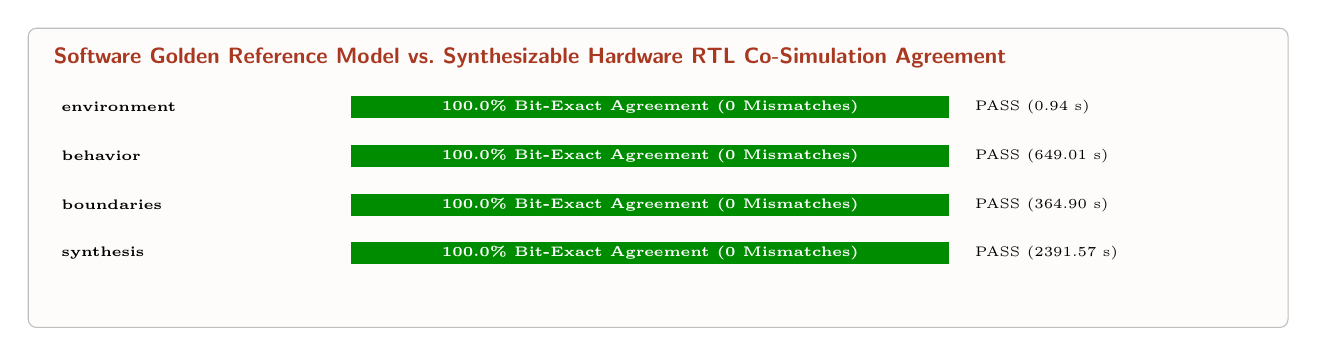
\begin{tikzpicture}[font=\scriptsize\sffamily]

\draw[draw=black!25,fill=vulcan!2,rounded corners=3pt] (-0.5,-1.85) rectangle (15.5,1.95);

\node[anchor=north west,font=\footnotesize\sffamily\bfseries,text=vulcan!90!black] at (-0.3,1.82) {Software Golden Reference Model vs.\ Synthesizable Hardware RTL Co-Simulation Agreement};

\node[anchor=west,font=\tiny\bfseries] at (-0.2,0.95) {environment};

\fill[green!55!black] (3.6,0.81) rectangle (11.2,1.09);

\node[text=white,font=\tiny\bfseries] at (7.4,0.95) {100.0\% Bit-Exact Agreement (0 Mismatches)};

\node[anchor=west,font=\tiny] at (11.4,0.95) {PASS (0.94 s)};

\node[anchor=west,font=\tiny\bfseries] at (-0.2,0.33) {behavior};

\fill[green!55!black] (3.6,0.19) rectangle (11.2,0.47);

\node[text=white,font=\tiny\bfseries] at (7.4,0.33) {100.0\% Bit-Exact Agreement (0 Mismatches)};

\node[anchor=west,font=\tiny] at (11.4,0.33) {PASS (649.01 s)};

\node[anchor=west,font=\tiny\bfseries] at (-0.2,-0.29) {boundaries};

\fill[green!55!black] (3.6,-0.43) rectangle (11.2,-0.15);

\node[text=white,font=\tiny\bfseries] at (7.4,-0.29) {100.0\% Bit-Exact Agreement (0 Mismatches)};

\node[anchor=west,font=\tiny] at (11.4,-0.29) {PASS (364.90 s)};

\node[anchor=west,font=\tiny\bfseries] at (-0.2,-0.91) {synthesis};

\fill[green!55!black] (3.6,-1.05) rectangle (11.2,-0.77);

\node[text=white,font=\tiny\bfseries] at (7.4,-0.91) {100.0\% Bit-Exact Agreement (0 Mismatches)};

\node[anchor=west,font=\tiny] at (11.4,-0.91) {PASS (2391.57 s)};

\end{tikzpicture}\par

{\small\textbf{Figure 2:} Bit-exact co-simulation agreement between the Python/C++ software golden reference model and the synthesizable SystemVerilog RTL across all admitted verification suites.}\end{center}

\subsection{Unified Hardware Signoff Gates (L1 Lint, L2 Quartus STA, L3 Physical FPGA)}

{\small\renewcommand{\arraystretch}{1.18}\begin{longtable}{@{}L{0.34\textwidth}L{0.12\textwidth}L{0.46\textwidth}@{}}\toprule

\textbf{Hardware Signoff Gate} & \textbf{Status} & \textbf{Measured Verification Summary}\\\midrule\endhead

L1 Static RTL Timing \& Synthesis Lint & PASSED & Combinational div/\allowbreak{}mod hazards: 0; mixed sequential assignments (\allowbreak{}10268)\allowbreak{}: 0\\[3pt]

\bottomrule\end{longtable}}

\section{Integration and use}

Use rtl/\allowbreak{}*\allowbreak{}.sv,\allowbreak{} design/\allowbreak{}SPEC.md,\allowbreak{} design/\allowbreak{}ARCHITECTURE.md and tests/\allowbreak{}*\allowbreak{} as deliverable inputs. Compile rivet\_\allowbreak{}a3\_\allowbreak{}pkg.sv before the other eleven RTL files and select rivet\_\allowbreak{}a3\_\allowbreak{}top. Adapted AES primitives are included; the read-only A2 reference is provenance,\allowbreak{} not a build dependency.


Assert reset low,\allowbreak{} keep input valids low,\allowbreak{} release reset and wait for post-release readiness. Load required keyslots and consume key results before dependent work. A suspended context binds its key until final retirement or successful abort.


Keep descriptors and source data stable while owned and prevent writable overlap between outstanding jobs. Supply one response for every accepted memory request,\allowbreak{} discard pre-reset responses and provide finite backpressure and response delays.


Use Python3.9 or newer,\allowbreak{} iverilog,\allowbreak{} vvp and Yosys on PATH. A focused clean reproduction is invoked from the delivered root by \texttt{python3 tests/\allowbreak{}verify.py --suite reproduce --output evidence/\allowbreak{}recipient-reproduce-001}; the destination must not exist. Suite commands are documented in design/\allowbreak{}SPEC.md and tests/\allowbreak{}README.md. Allocate fresh destinations rather than reusing recorded output paths.


The synthesis helper handles Yosys0.33 package-import limitations by inserting the verbatim package body into generated inputs; functional simulation uses unchanged package/\allowbreak{}import RTL. Compressed complete netlists,\allowbreak{} raw logs and source-bound receipts reside under the recorded suite outputs.


\section{Limitations and acceptance boundary}

This delivery establishes verified RTL and default-capacity generic synthesis,\allowbreak{} not placement/\allowbreak{}routing,\allowbreak{} technology-specific timing,\allowbreak{} frequency,\allowbreak{} power,\allowbreak{} silicon area,\allowbreak{} FPGA operation or fabrication sign-off.


The byte-serial memory adapter and shared engines prioritize explicit ownership and correctness. No fixed latency,\allowbreak{} sustained throughput or fairness bound is claimed; continuous high-priority traffic may starve normal work.


GCM uses96-bit IVs and full128-bit tags. Software must provide unique IVs. Hardware nonce-reuse prevention,\allowbreak{} side-channel hardening and cryptographic certification are not claimed.


Simulation and structural zeroization checks are bounded,\allowbreak{} not exhaustive formal proof. Maximum-capacity synthesis and a full capacity256 seeded campaign were not established.


Memory errors cannot undo acknowledged writes. Authentication failure prevents payload writes,\allowbreak{} but late transport failures can leave partial output. Software must inspect completion status before treating destination contents as successful.


\appendix\section{Source inventory}

Production inventory: 12 Verilog/\allowbreak{}SystemVerilog files; 1548 nonblank,\allowbreak{} non-comment lines. Source size is not a correctness or quality metric.

{\small\renewcommand{\arraystretch}{1.18}\begin{longtable}{@{}L{0.61\textwidth}L{0.15\textwidth}L{0.15\textwidth}@{}}\toprule

\textbf{Production file} & \textbf{Physical lines} & \textbf{Code lines}\\\midrule\endhead

rtl/\allowbreak{}rivet\_\allowbreak{}a3\_\allowbreak{}aes\_\allowbreak{}core.sv & 48 & 45\\[3pt]

rtl/\allowbreak{}rivet\_\allowbreak{}a3\_\allowbreak{}context\_\allowbreak{}store.sv & 22 & 22\\[3pt]

rtl/\allowbreak{}rivet\_\allowbreak{}a3\_\allowbreak{}datapath.sv & 86 & 81\\[3pt]

rtl/\allowbreak{}rivet\_\allowbreak{}a3\_\allowbreak{}ghash.sv & 63 & 61\\[3pt]

rtl/\allowbreak{}rivet\_\allowbreak{}a3\_\allowbreak{}key\_\allowbreak{}schedule.sv & 90 & 86\\[3pt]

rtl/\allowbreak{}rivet\_\allowbreak{}a3\_\allowbreak{}key\_\allowbreak{}table.sv & 59 & 59\\[3pt]

rtl/\allowbreak{}rivet\_\allowbreak{}a3\_\allowbreak{}mixcolumns.sv & 24 & 23\\[3pt]

rtl/\allowbreak{}rivet\_\allowbreak{}a3\_\allowbreak{}pkg.sv & 105 & 97\\[3pt]

rtl/\allowbreak{}rivet\_\allowbreak{}a3\_\allowbreak{}sbox.sv & 15 & 14\\[3pt]

rtl/\allowbreak{}rivet\_\allowbreak{}a3\_\allowbreak{}scheduler\_\allowbreak{}dma.sv & 263 & 263\\[3pt]

rtl/\allowbreak{}rivet\_\allowbreak{}a3\_\allowbreak{}shiftrows.sv & 17 & 16\\[3pt]

rtl/\allowbreak{}rivet\_\allowbreak{}a3\_\allowbreak{}top.sv & 783 & 781\\[3pt]

\bottomrule\end{longtable}}

\section{Verification record index}

{\small\renewcommand{\arraystretch}{1.18}\begin{longtable}{@{}L{0.57\textwidth}L{0.16\textwidth}L{0.17\textwidth}@{}}\toprule

\textbf{Recorded check} & \textbf{Outcome} & \textbf{Execution time (\allowbreak{}s)\allowbreak{}}\\\midrule\endhead

environment & passed & 0.941\\[3pt]

behavior & passed & 649.009\\[3pt]

boundaries & passed & 364.900\\[3pt]

synthesis & passed & 2391.567\\[3pt]

checker\_\allowbreak{}sensitivity & passed & 2.660\\[3pt]

clean\_\allowbreak{}reproduction & passed & 68.002\\[3pt]

recovery-002-environment & passed & 0.966\\[3pt]

recovery-002-behavior & passed & 652.063\\[3pt]

recovery-002-boundaries & passed & 364.392\\[3pt]

recovery-002-synthesis & passed & 2373.040\\[3pt]

recovery-002-checker-sensitivity & passed & 2.676\\[3pt]

recovery-002-clean-reproduction & passed & 67.148\\[3pt]

\bottomrule\end{longtable}}

Execution times include tool and provider waiting; they are not hardware latency or model utilization.

{\small\renewcommand{\arraystretch}{1.18}\begin{longtable}{@{}L{0.12\textwidth}L{0.82\textwidth}@{}}\toprule

\textbf{Reference} & \textbf{Original project-relative record}\\\midrule\endhead

E019 & tests/\allowbreak{}boundary\_\allowbreak{}units.sv\\[3pt]

E020 & tests/\allowbreak{}bridge.sv\\[3pt]

E021 & tests/\allowbreak{}oracle.py\\[3pt]

E022 & tests/\allowbreak{}scenarios.py\\[3pt]

E023 & tests/\allowbreak{}test\_\allowbreak{}runner.py\\[3pt]

E024 & tests/\allowbreak{}verify.py\\[3pt]

E033 & .vulcan/\allowbreak{}engineering/\allowbreak{}run-0001/\allowbreak{}attempt-0006/\allowbreak{}stdout.log\\[3pt]

E035 & .vulcan/\allowbreak{}engineering/\allowbreak{}run-0001/\allowbreak{}attempt-0008/\allowbreak{}stdout.log\\[3pt]

E1062 & .vulcan/\allowbreak{}engineering/\allowbreak{}run-0002/\allowbreak{}attempt-0003/\allowbreak{}stdout.log\\[3pt]

E1063 & .vulcan/\allowbreak{}engineering/\allowbreak{}run-0002/\allowbreak{}attempt-0004/\allowbreak{}stdout.log\\[3pt]

E1064 & .vulcan/\allowbreak{}engineering/\allowbreak{}run-0002/\allowbreak{}attempt-0005/\allowbreak{}stdout.log\\[3pt]

E1065 & .vulcan/\allowbreak{}engineering/\allowbreak{}run-0002/\allowbreak{}attempt-0006/\allowbreak{}stdout.log\\[3pt]

E1066 & .vulcan/\allowbreak{}engineering/\allowbreak{}run-0002/\allowbreak{}attempt-0007/\allowbreak{}stdout.log\\[3pt]

E1067 & .vulcan/\allowbreak{}engineering/\allowbreak{}run-0002/\allowbreak{}attempt-0008/\allowbreak{}stdout.log\\[3pt]

E1069 & .vulcan/\allowbreak{}engineering/\allowbreak{}run-0002/\allowbreak{}attempt-0010/\allowbreak{}stdout.log\\[3pt]

E1070 & .vulcan/\allowbreak{}engineering/\allowbreak{}run-0002/\allowbreak{}attempt-0011/\allowbreak{}stdout.log\\[3pt]

E1071 & .vulcan/\allowbreak{}engineering/\allowbreak{}run-0002/\allowbreak{}attempt-0012/\allowbreak{}stdout.log\\[3pt]

E1072 & .vulcan/\allowbreak{}engineering/\allowbreak{}run-0002/\allowbreak{}attempt-0013/\allowbreak{}stdout.log\\[3pt]

E1073 & .vulcan/\allowbreak{}engineering/\allowbreak{}run-0002/\allowbreak{}attempt-0014/\allowbreak{}stdout.log\\[3pt]

\bottomrule\end{longtable}}

\section{Document provenance}

Engineering was independently accepted for the recorded source and evidence identity. This is not exhaustive proof, hardware deployment or physical signoff. The companion REPORT.md records the exact report approval and source manifest, and links the English/Chinese journeys containing original failures and interventions. A report number identifies a generation attempt, not a new hardware revision.

Developer attribution is explicitly supplied project metadata, not inferred affiliation or institutional endorsement.

\end{document}
